\chapter{Анализ текущей системы межсервисной авторизации и выявление ее ограничений}\label{ch:1}

% PLAN. DO NOT REMOVE FROM THIS DOC.
% 1. Описание текущего устройства микросервисной авторизации в Mindbox (обязательно с mermaid диаграммами).
% 2. Проблема описанной авторизации.
% 3. Формирование технических требований для перехода на безопасную авторизацию в контексте Mindbox.
% 4. Анализ существующих систем авторизации с автоматической ротацией ключа. Должно приводить к выводу, что ничего для наших требований не подойдет, разрабатываем сами.
% 5. Исследование научных работ на аспекты текущей работы:
% - mTLS + Istio + SPIFFE. Здесь надо прийти, что это очень круто, но такая миграция займет много времени + у команды нет технических навыков SRE.
% - JWT. В целом что это такое, их каких частей состоит, как используется для чего. Какие проблемы есть. Про то, что его сложно отзывать, как с этим бороться.
% - Исследования на тему бесшовной ротации. Как делают, grace period и т.п.
% - Способы подписания токенов. RSA (особенно про размер ключа в 2030 годах, что он должен быть минимум 3192 или что-то такое).
% - Token Exchange. Как другие системы его делают, какие есть риски. Федерация систем авторизации.
% - OIDC. Для чего нужен, какие проблемы решает.
% - IaC. Что такое, как используется, преимущества недостатки.
% 6. Выделение критериев сравнения и подбор инструментальных средств на их основе
% - База данных: PostgreSQL
% - Хранилище ключей: Vault
% - Распределенный кэш: Dragonfly
% - Языки программирования: C# для микросервиса и библиотеки, Go для k8s оператора и Terraform Provider
% 7. Формулирование задачи и гипотезы ее решения
% 8. Выводы по главе

\section{Текущее устройство микросервисной авторизации}\label{sec:current-auth}

\subsection{Микросервисная мультитенантная архитектура}\label{subsec:arch}

Платформа Mindbox представляет собой мультитенантную микросервисную систему,
насчитывающую порядка 120 независимо развёртываемых сервисов.
Клиентами (тенантами) платформы являются компании, использующие Mindbox
для автоматизации маркетинга и роста своего бизнеса, ~--- например, Яндекс Образование, Купер, СДЭК и другие.
Каждый сервис обслуживает запросы разных тенантов одновременно, разделяя данные на уровне приложения
за счет добавления идентификатора клиента в claim \texttt{tenant} JWT-токена.
Единственным исключением является CDP (Customer Data Platform)~---
административная панель клиента, которая развёртывается для каждого тенанта отдельно,
однако при обработке запросов обращается к общим мультитенантным микросервисам (\firef{fig:cdp-microservices}).

Инструментарий для работы с авторизацией централизованно реализован
в библиотеке \texttt{Mindbox.Authentication}.
Она предоставляет единый набор функций для генерации и проверки JWT-токенов
и используется всеми микросервисами платформы.

\begin{figure}[h]
  \centering
  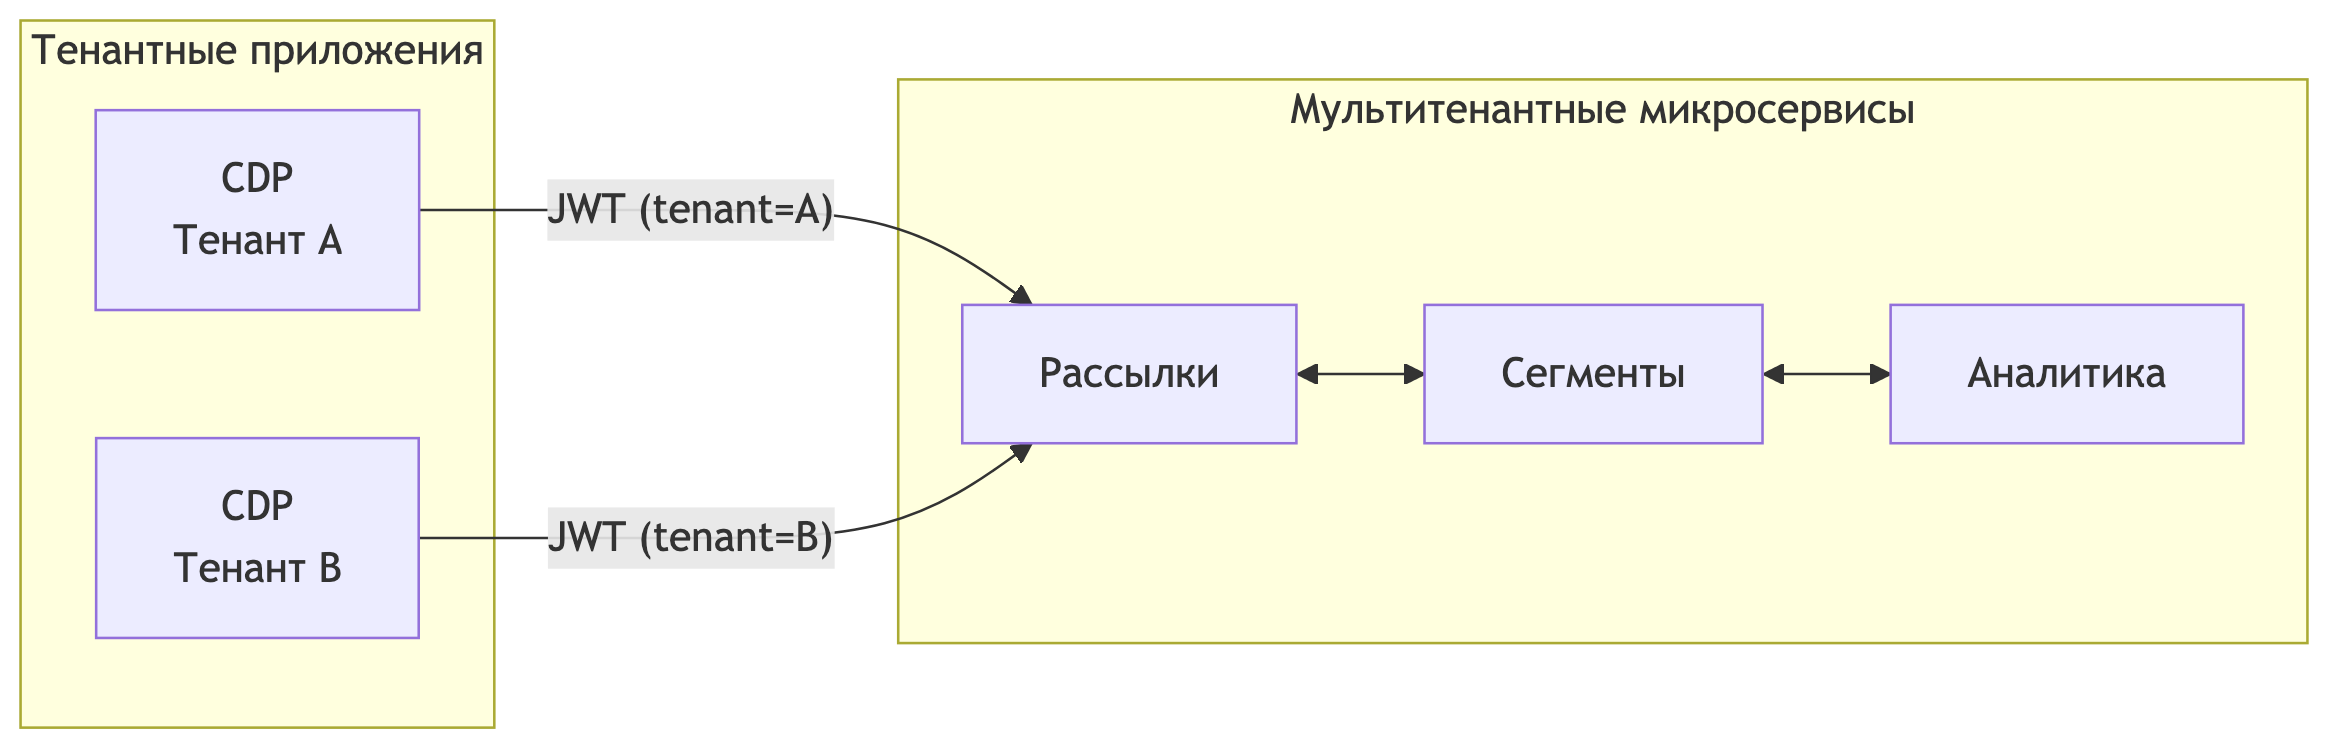
\includegraphics[width=0.8\textwidth]{diagrams/img/ch1_cdp_microservices}
  \caption{Взаимодействие тенантных CDP и мультитенантных микросервисов}
  \label{fig:cdp-microservices}
\end{figure}

\subsection{Контуры развёртывания}\label{subsec:contours}

Для обеспечения изоляции сред и управления рисками при развёртывании платформа разделена на несколько контуров.

\begin{itemize}
  \item \textbf{Alpha} (Staging)~--- среда разработчиков.
    Предназначена для локальной отладки и интеграционного тестирования до попадания изменений на боевые контуры.
    Использует собственный набор криптографических ключей, изолированный от остальных контуров.
  \item \textbf{Beta}~--- контур предрелизного тестирования на ограниченной группе реальных пользователей.
    Позволяет выявить дефекты в условиях, приближённых к боевой эксплуатации, до масштабного развёртывания.
  \item \textbf{Gamma} (Stable)~--- основное боевое окружение,
    обслуживающее подавляющее большинство клиентов и принимающее максимальную нагрузку.
    Именно на этом контуре обрабатывается свыше 2 миллионов запросов в минуту.
  \item \textbf{Sigma}~--- дополнительный боевой контур, функционально аналогичный Gamma.
    Создан для размещения новых клиентов и дальнейшего масштабирования платформы.
  \item \textbf{Omega}~--- полностью изолированный боевой контур,
    развёрнутый в облачной инфраструктуре AWS\@.
  \item \textbf{Infra}~--- внутренний инфраструктурный контур компании.
    Содержит инструменты администрирования проектами клиентов (CDP приложения)
    на всех вышеперечисленных контурах.
\end{itemize}

\subsection{Изолированность контуров}\label{subsec:contour-isolation}

Несмотря на архитектурное разделение,
изоляция между контурами умышленно нарушается в нескольких точках (\firef{fig:contour-interaction}).
Контур infra по своему назначению коммуницирует со всеми остальными контурами,
и наоборот~--- сервисы на боевых контурах отправляют запросы к infra для выполнения административных операций.

\begin{figure}[h]
  \centering
  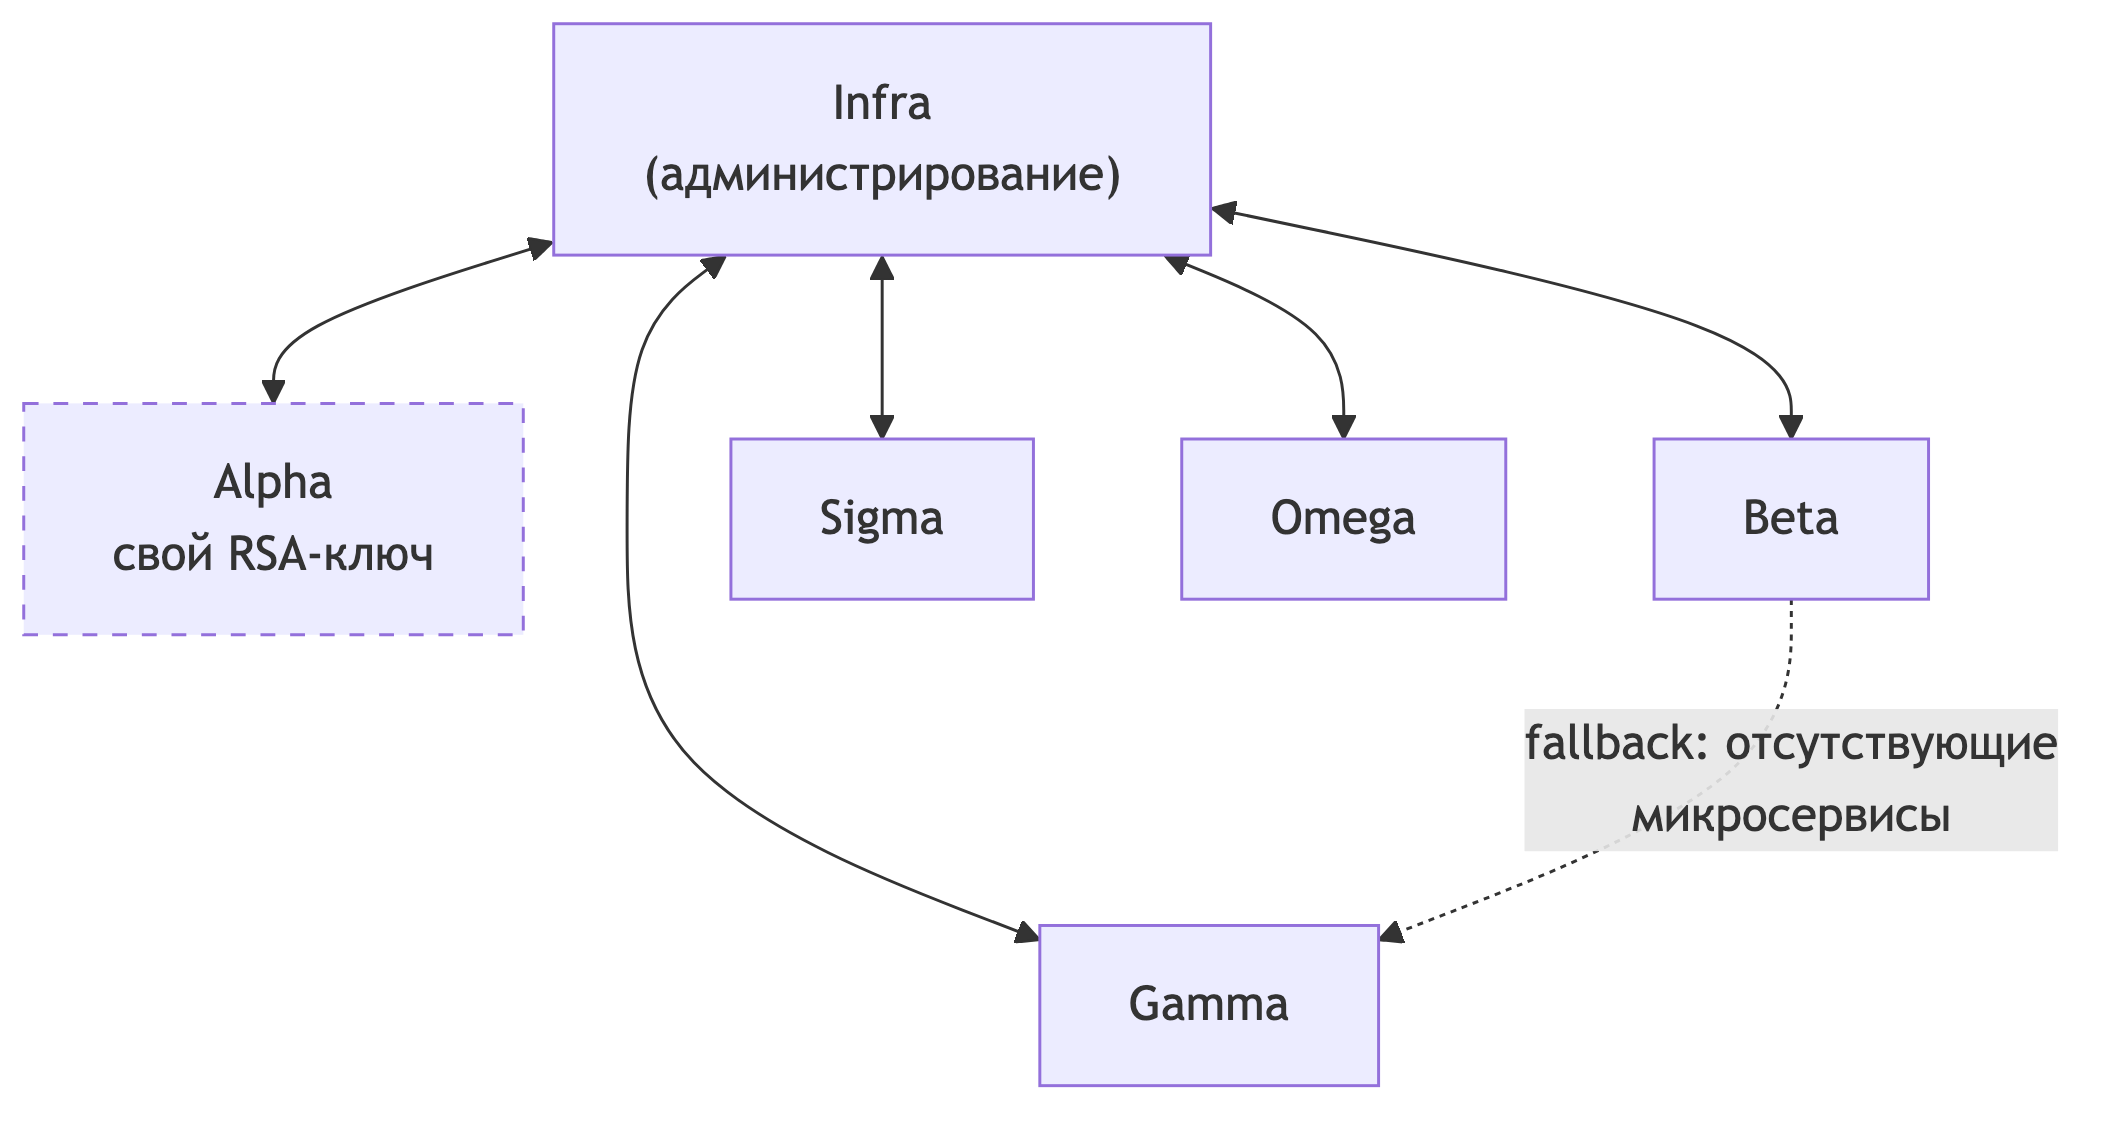
\includegraphics[width=0.6\textwidth]{diagrams/img/ch1_contour_interaction}
  \caption{Схема взаимодействия между контурами развёртывания}
  \label{fig:contour-interaction}
\end{figure}

Кроме того, часть микросервисов отсутствует на контуре beta.
В таких случаях запросы с Beta перенаправляются на Gamma, образуя межконтурный fallback-маршрут.

Наиболее критичным с точки зрения безопасности является то,
что на всех контурах, кроме Alpha, используется \textbf{один и тот же закрытый RSA-ключ}
для подписи и верификации JWT-токенов.
Таким образом, компрометация ключа на любом из контуров автоматически ставит под угрозу все остальные.
Единый ключ порождает неявное межконтурное взаимодействие:
токен, выпущенный на одном контуре, валиден на любом другом,
и по самому токену невозможно определить, для какого контура он предназначен.
Это упрощает эксплуатацию,
однако при проектировании новой системы авторизации станет одной из ключевых сложностей~---
ротация ключа на одном контуре не должна нарушать работу остальных.

\subsection{Текущая схема JWT-авторизации}\label{subsec:jwt-scheme}

Для хранения секретов платформа использует HashiCorp Vault~\cite{HashiCorpVault}~---
систему централизованного управления секретами.
Все 120 микросервисов имеют доступ к закрытому RSA-ключу, хранящемуся в Vault.
Централизованного контроля над выпуском токенов не существует~---
на практике сложились два разрозненных подхода к работе с JWT\@.

\begin{enumerate}
  \item \textbf{Статические токены в Vault.}
    Для межсервисного взаимодействия, не требующего динамических данных из рантайма,
    разработчик вручную генерирует JWT, подписывает его закрытым ключом и сохраняет в Vault как секрет.
    Чтобы избежать повторной ручной генерации,
    срок действия таких токенов устанавливается в 10 лет.
    В рантайме сервис просто считывает готовый токен из Vault
    и использует его для запросов (\firef{fig:static-jwt}).

    \begin{figure}[h]
      \centering
      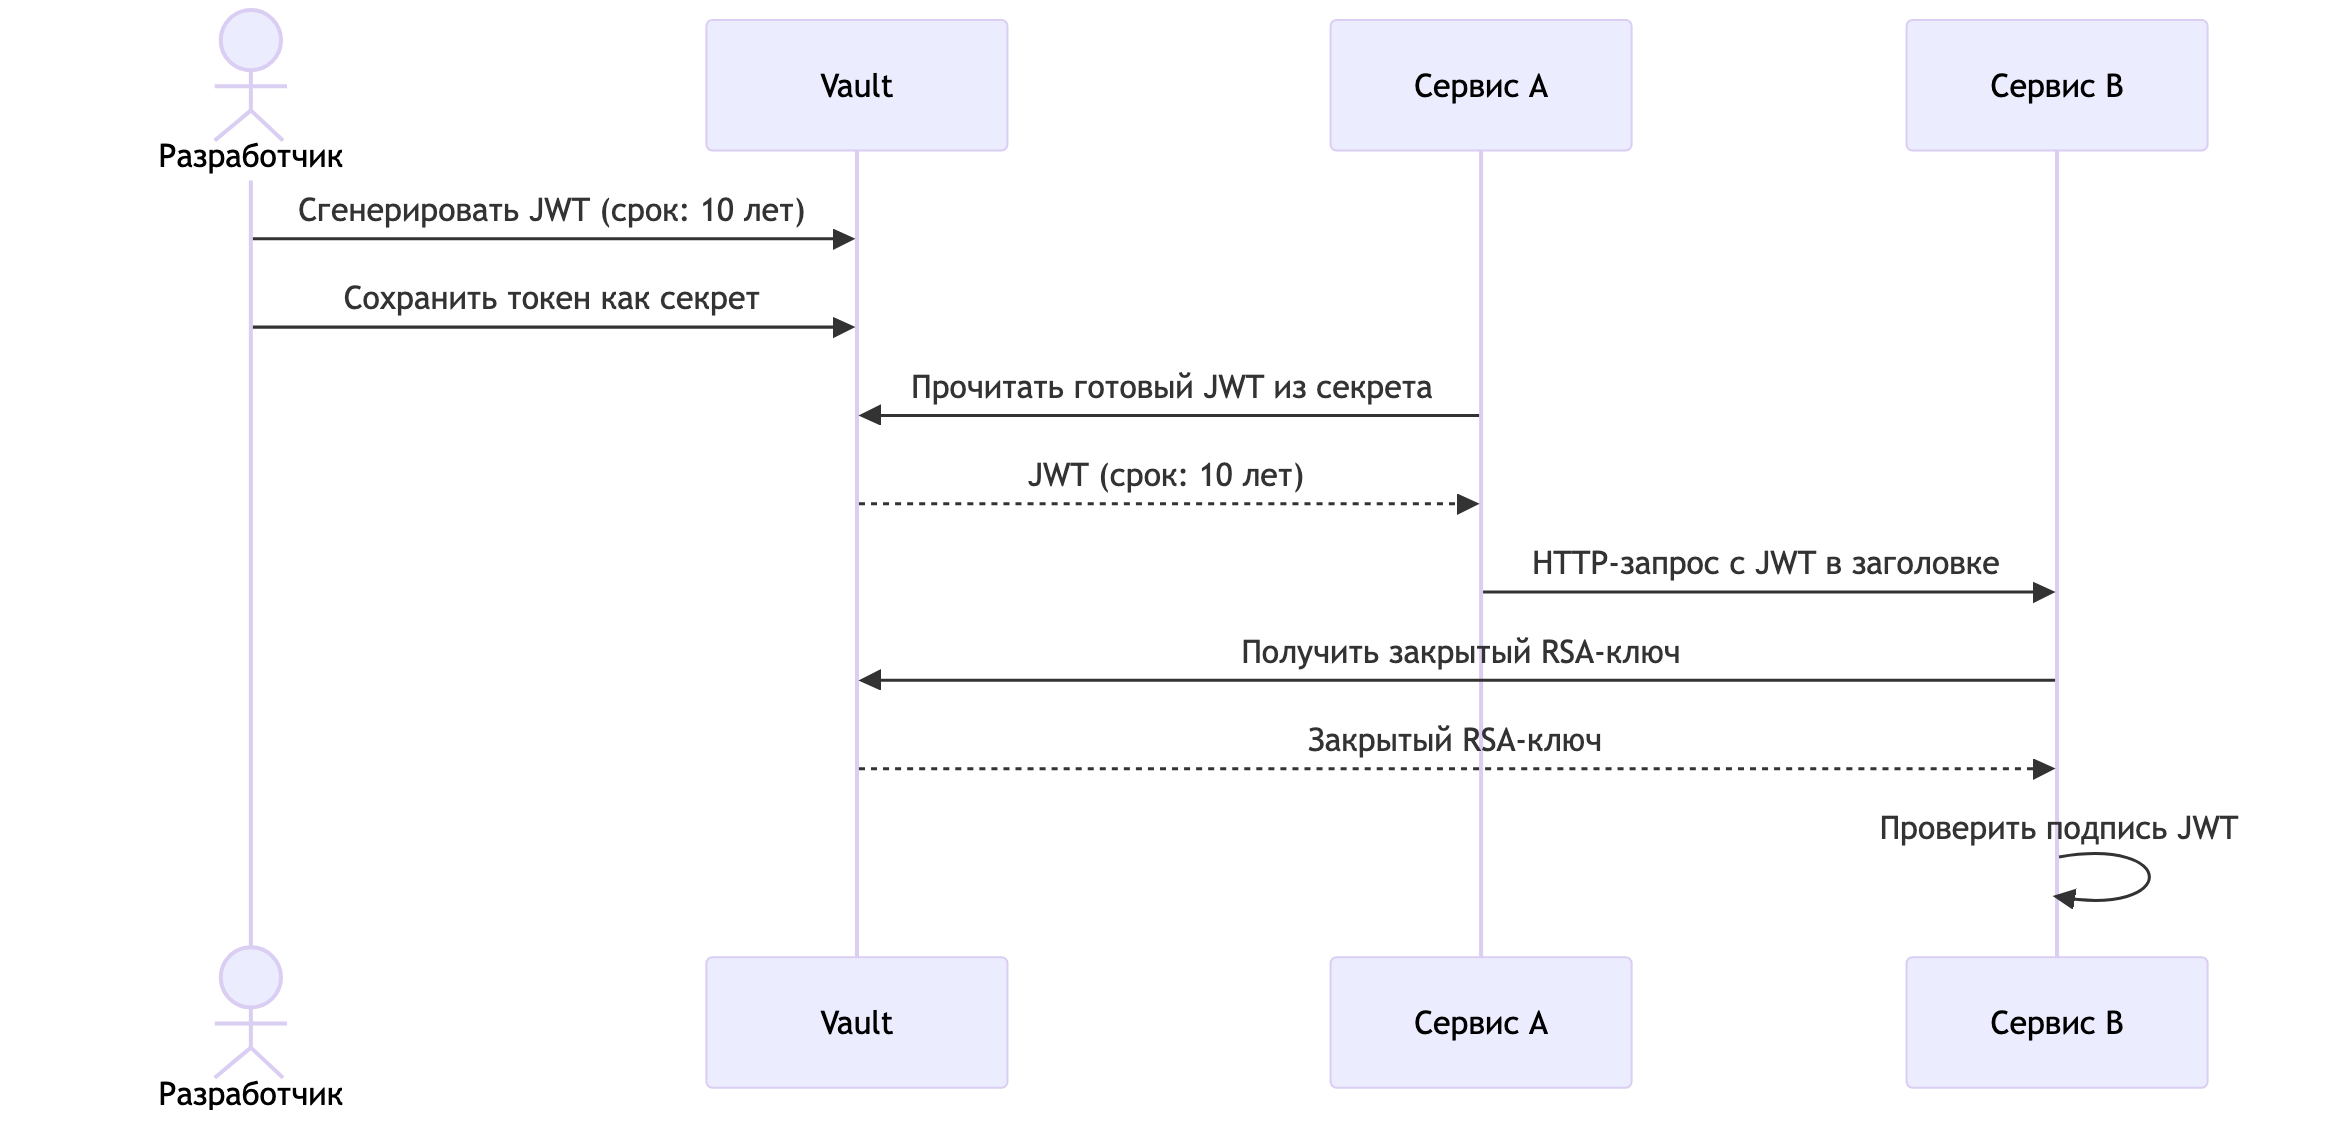
\includegraphics[width=0.85\textwidth]{diagrams/img/ch1_static_jwt}
      \caption{Использование статического JWT-токена из Vault}
      \label{fig:static-jwt}
    \end{figure}

  \item \textbf{Динамическая генерация.}
    Когда в токен необходимо включить данные, известные только в момент запроса
    (например, идентификатор тенанта или пользователя),
    сервис самостоятельно получает закрытый ключ из Vault
    и подписывает JWT в рантайме.
    Этот подход применяется прежде всего для пользовательских токенов
    (\firef{fig:dynamic-jwt}).

    \begin{figure}[h]
      \centering
      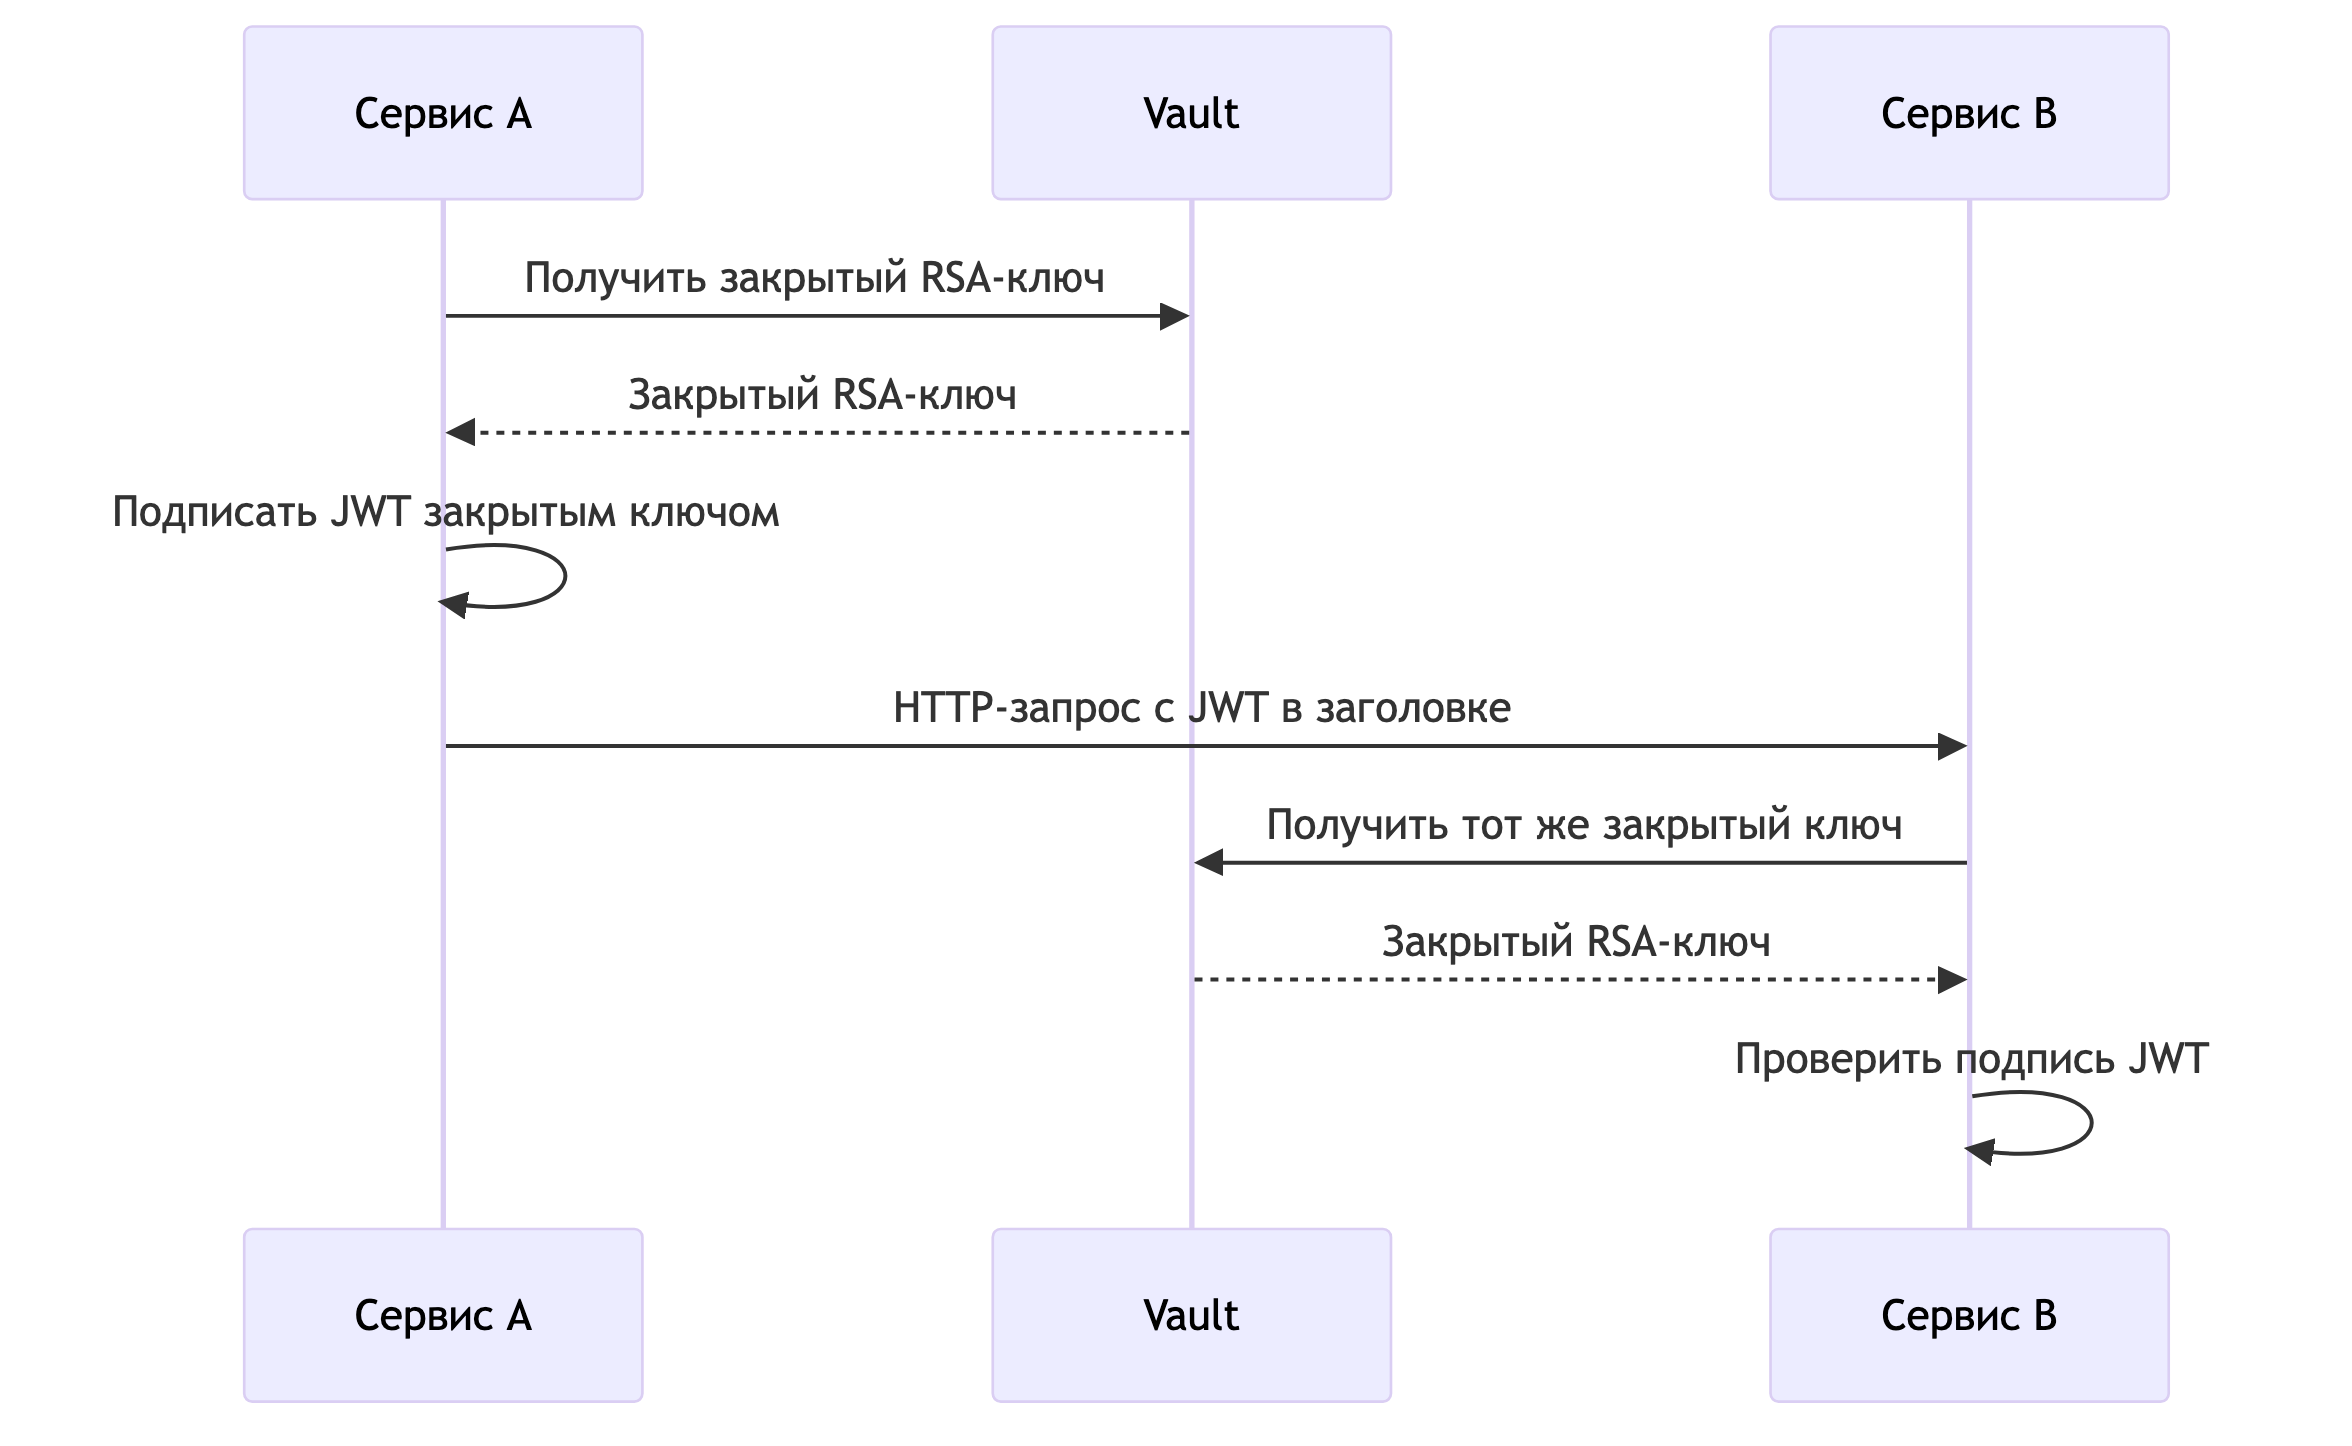
\includegraphics[width=0.85\textwidth]{diagrams/img/ch1_dynamic_jwt}
      \caption{Динамическая генерация JWT в рантайме}
      \label{fig:dynamic-jwt}
    \end{figure}
\end{enumerate}

Однако граница между двумя подходами не контролируется:
любой микросервис имеет доступ к закрытому ключу
и может выпустить произвольный токен~--- как сервисный, так и пользовательский.
Схема авторизации не разделяет эти типы токенов: они имеют одинаковую структуру.

Помимо микросервисов, JWT-токены Mindbox используются сторонними системами:
платформой автоматизации Make, системой управления конфигурацией Ansible,
оркестратором развёртывания Octopus Deploy и CI/CD-системой GitLab.
Эти внешние потребители также хранят долгоживущие токены
и должны быть учтены при проектировании механизма ротации.

Описанная схема отличается простотой и удобством для разработчиков:
низкий порог входа и отсутствие централизованного сервиса авторизации
позволяли командам быстрыми темпами развивать продукт.
Однако по мере роста платформы те же свойства превратились
в архитектурные ограничения и угрозы безопасности,
мотивирующие переход к новой системе авторизации.
